\documentclass[a4paper, 12pt]{article}
\usepackage{amsmath}
\usepackage{graphicx}
\usepackage{float}
\usepackage{geometry}
\geometry{a4paper, top=25mm, left=25mm, right=25mm, bottom=25mm}

\begin{document}

\title{Cepheiden und die galaktische Entfernungsskala}
\author{Guilherme Schmid}
\date{Sommersemester 2024}
\maketitle

\section{Zielsetzung}
Das Ziel des Versuchs war es, den Abstand von Cepheiden in der Kleinen Magellanschen Wolke (SMC) zu bestimmen. Diese Bestimmung erfolgt durch die Analyse der Periode und Helligkeiten der Cepheiden, die Berechnung der absoluten Helligkeiten und schließlich die Berechnung der Entfernung zur SMC.

\section{Durchführung und Auswertung}

\subsection{Bestimmung der Periode und Helligkeiten}
Die Perioden \( P \), maximalen Helligkeiten \( m_{\text{max}} \) und minimalen Helligkeiten \( m_{\text{min}} \) der Cepheiden wurden aus den Lichtkurven bestimmt. Die mittlere scheinbare Helligkeit \( m \) wurde berechnet als:
\begin{equation}
    m = \frac{1}{2} (m_{\text{max}} + m_{\text{min}})
\end{equation}

\subsection{Berechnung von \(\log P\) und \(m\)}
Die Periode wurde in den logarithmischen Wert \(\log P\) umgerechnet.

\subsection{Erstellung des \(\log P - m\)-Diagramms}
Die in Tabelle 4.1 und 4.2 gegebenen Wertepaare sowie die neu bestimmten Cepheiden wurden in einem \(\log P - m\)-Diagramm dargestellt. Für beide Datengruppen wurde eine Ausgleichsgerade bestimmt, um die Beziehung zwischen \(\log P\) und \(m\) bzw. \(M\) darzustellen.

\begin{figure}[H]
    \centering
    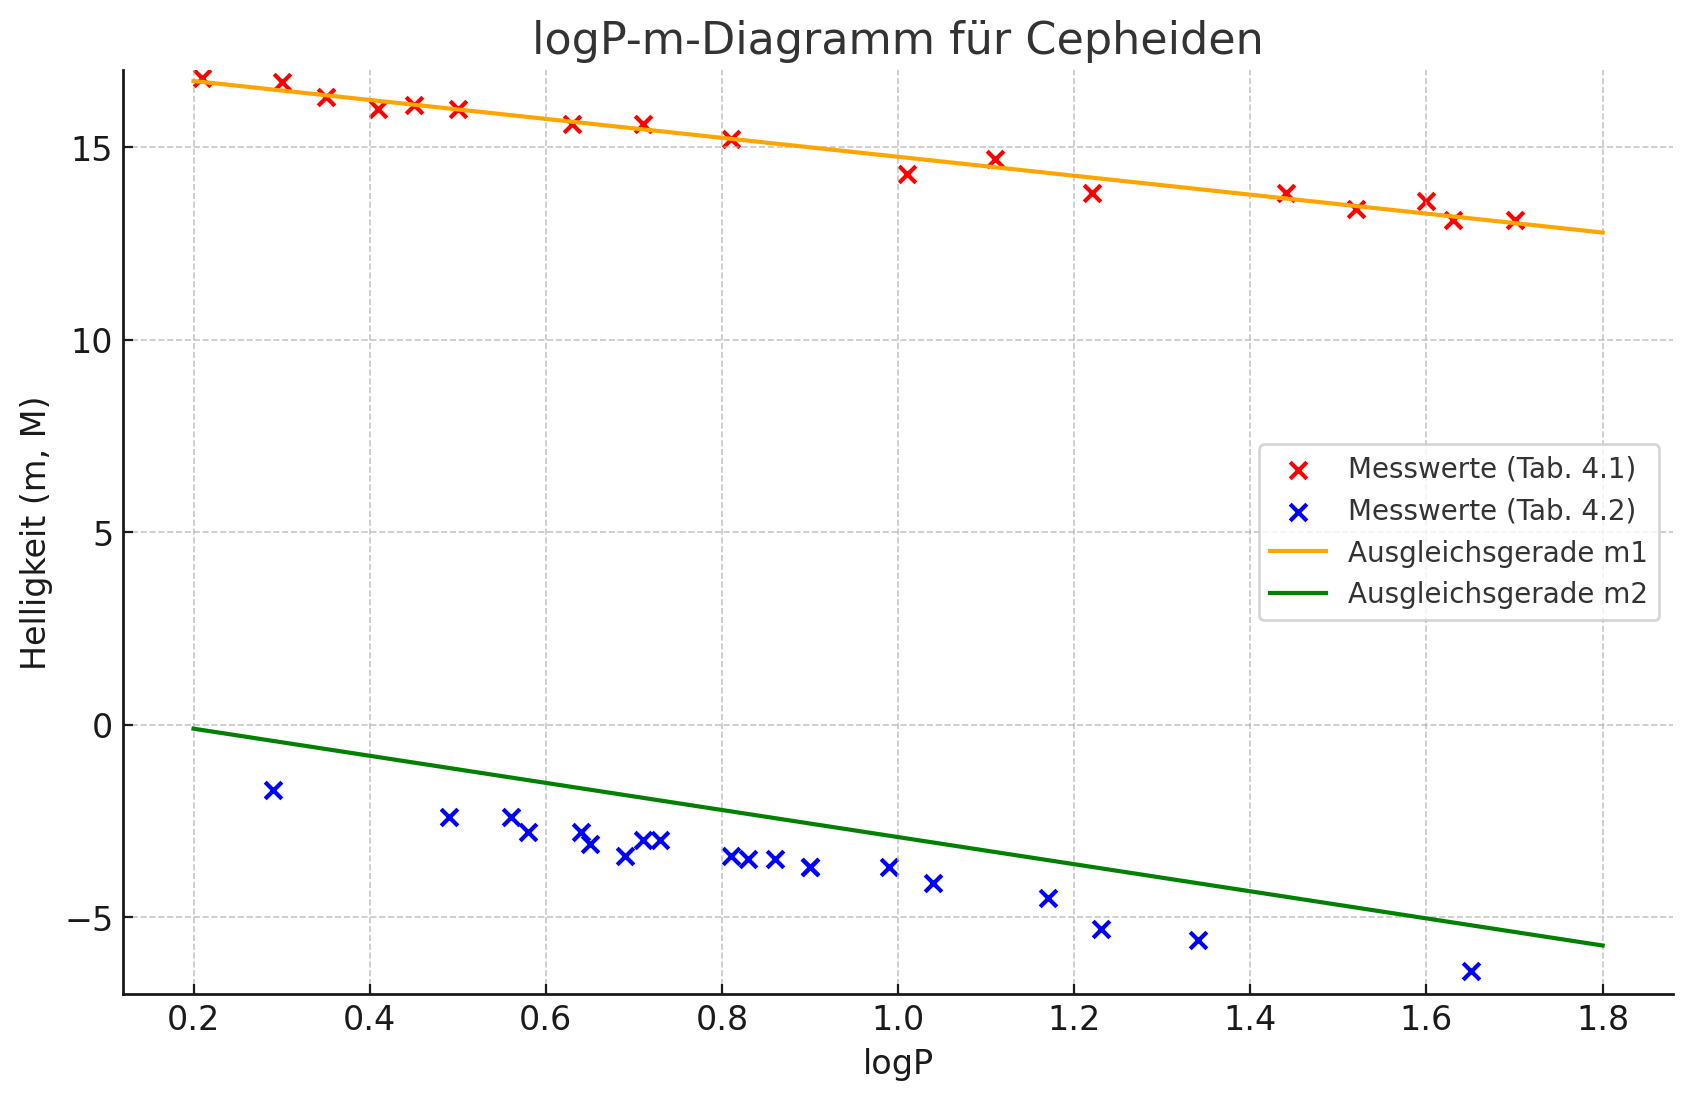
\includegraphics[width=0.8\textwidth]{plot.png} % Pfad zum Diagramm anpassen
    \caption{\(\log P - m\)-Diagramm für Cepheiden}
    \label{fig:logP-m}
\end{figure}

\subsection{Bestimmung des Abstands \(m - M\)}
Der Abstand \(m - M\) wurde für \(\log P = 0\) und \(\log P = 2\) berechnet und gemittelt, um die Helligkeitsdifferenz zu bestimmen.

\subsection{Berechnung der Entfernung \(d\) zur SMC}
Die Entfernung \(d\) wurde mit der folgenden Formel berechnet:
\begin{equation}
    d = 10^{\frac{m - M + 5}{5}} \text{ pc}
\end{equation}
Die Helligkeitsdifferenz \(m - M\) beträgt etwa 18.63, was zur berechneten Entfernung von 53.12 kpc führt. Bei einer Korrektur der absoluten Helligkeit \(M\) um 1.5 ergibt sich eine Entfernung von etwa 26.62 kpc.

\section{Fazit}
Die Entfernung zur Kleinen Magellanschen Wolke (SMC) wurde erfolgreich berechnet. Diese Berechnungen zeigen, wie empfindlich die Entfernungsbestimmung gegenüber Änderungen in den Helligkeitsparametern ist.
\section*{Anhang}
Die Berechnungen wurden mit Hilfe eines Python-Skripts durchgeführt, welches die erforderlichen Messdaten und Berechnungen automatisiert hat.

\end{document}
